\documentclass[11pt, oneside]{article}
\usepackage[letterpaper, margin=2cm]{geometry}
\usepackage{MATH565}
\usepackage{xspace}
\newcommand{\MATLAB}{\textsc{Matlab}\xspace}
\newcommand{\PYTHON}{\textsc{Python}\xspace}

\begin{document}
\noindent \textbf{\Large{Caleb Logemann \\
MATH 565 Continuous Optimization \\
Homework 1
}}

%\lstinputlisting[language=Python]{H01_23.m}
\begin{enumerate}
  \item % #1 Done
    Problem 1 \\
    Compute the gradient $\nabla f(x)$ and Hessian $\nabla^2 f(x)$ of the
    Rosenbrock function
    \[
      f(x) = 100\p{x_2 - x_1^2}^2 + (1 - x_1)^2
    \]

    The gradient of $f$ is defined as $\p{\pd{f}{x_1}, \pd{f}{x_2}}^T$.
    The first derivatives of $f$ are stated below.
    \begin{align*}
      \pd{f}{x_1} &= -400 x_1 \p{x_2 - x_1^2} - 2(1 - x_1) \\
      \pd{f}{x_2} &= 200\p{x_2 - x_1^2}
    \end{align*}
    So the gradient of $f$ is 
    \[
      \nabla f(x) =
      \begin{bmatrix}
        -400 x_1 \p{x_2 - x_1^2} - 2(1 - x_1) \\
        200\p{x_2 - x_1^2}
      \end{bmatrix}
    \]
    The Hessian of $f$ is the matrix
    \[
      \nabla^2 f(x) =
      \begin{bmatrix}
        \pd[2]{f}{x_1} & \mpd[2]{f}{\partial x_1 \partial x_2} \\
        \mpd[2]{f}{\partial x_2 \partial x_1} & \pd[2]{f}{x_2}
      \end{bmatrix}
    \]
    The second derivatives are shown below.
    \begin{align*}
      \pd[2]{f}{x_1} &= \pda{}{x_1}{\pd{f}{x_1}} \\
      &= -400\p{x_2 - x_1^2} + 800 x_1^2 + 2 \\
      &= -400\p{x_2 - 3x_1^2} + 2 \\
      \mpd[2]{f}{\partial x_1 \partial x_2} &= \pda{}{x_1}{\pd{f}{x_2}} \\
      &= -400 x_1 \\
      \pd[2]{f}{x_2} &= \pda{}{x_2}{\pd{f}{x_2}} \\
      &= 200
    \end{align*}
    Note that $\mpd[2]{f}{\partial x_2 \partial x_1} = \mpd[2]{f}{\partial x_1 \partial x_2}$
    as $f$ has continuous second derivatives.
    Thus the Hessian of $f$ is 
    \[
      \nabla^2 f(x) =
      \begin{bmatrix}
         -400\p{x_2 - 3x_1^2} + 2 & -400x_1 \\
        -400x_1 & 200
      \end{bmatrix}
    \]

  \item % #2 Done
    Problem 8 \\
    Suppose that $f$ is a convex function.
    Show that the set of global minimizers of $f$ is a convex set.

    \begin{proof}
      Let $f$ be a convex function.
      This implies that
      \[
        f(\lambda x + (1 - \lambda) y) \le \lambda f(x) + (1 - \lambda) f(y)
      \]
      for $\lambda \in \br{0, 1}$ and $x, y \in \RR^n$.
      Let $S = \set{x^* \in \RR^n : f(x^*) \le f(x) \forall x \in \RR^n}$ be
      the set of all global minimizers.
      Let $x_1^*, x_2^* \in S$ and let $\lambda \in \br{0, 1}$.
      Note that $f(x_1^*) = f(x_2^*)$ because in order for both of these to be
      global minimizers they must have the same functional value.
      Now consider the point $\lambda x_1^* + (1-\lambda)x_2^*$.
      Since $f$ is convex.
      \begin{align*}
        f(\lambda x_1^* + (1-\lambda)x_2^*) &\le \lambda f(x_1^*) + (1 - \lambda) f(x_2^*) \\
        &= \lambda f(x_1^*) + (1 - \lambda) f(x_1^*) \\
        &= f(x_1^*) \\
      \end{align*}
      This shows tha
      Also since $x_1^*$ is a global minimizer.
      \[
        f(\lambda x_1^* + (1-\lambda)x_2^*) \le f(x_1^*) \le f(x)
      \]
      for any $x \in \RR^n$.
      Thus $\lambda x_1^* + (1 - \lambda)x_2^* \in S$ and is a global minimizer.
      This shows that $S$ is convex.
    \end{proof}

  \item % #3 Done
    Problem 9 \\
    Consider the function $f(x_1, x_2) = (x_1 + x_2^2)^2$.
    At the point $x^T = (1, 0)$ we consider the search direction $p^T = (-1, 1)$.
    Show that $p$ is a descent direction and find all minimizers of the problem
    (2.10).

    In order to show that this is a descent direction, it is first necessary to
    find the gradient of $f$ at $x^T = (1, 0)$.
    \[
      \nabla f =
      \begin{bmatrix}
        2(x_1 + x_2^2) \\
        4x_2(x_1 + x_2^2)
      \end{bmatrix}
    \]
    At the point $x^T = (1, 0)$, the gradient is
    \[
      \nabla f(x) =
      \begin{bmatrix}
        2 \\
        0
      \end{bmatrix}
    \]
    This is a descent direction if $p^T \nabla f(x) < 0$.
    Now note that $p^T \nabla f(x) = (-1)\times 2 + 1 \times 0 = -2 < 0$.
    Therefore $p$ is a descent direction.

    Secondly we want to find the minimizers of the problem.
    \[
      \min[\alpha > 0]{f(x + \alpha p)} = \min[\alpha > 0]{\phi(\alpha)}
    \]
    We can find the vector $x + \alpha p$ to be
    \[
      x + \alpha p =
      \begin{bmatrix}
        1 - \alpha \\
        \alpha
      \end{bmatrix}
    \]
    Now the function $\phi(\alpha)$ can be given as
    \[
      \phi(\alpha) = (1 - \alpha + \alpha^2)^2
    \]
    In order to find the minimizers of this function we must first find the
    derivative of $\phi$.
    \[
      \phi'(\alpha) = 2(\alpha^2 - \alpha + 1)(2\alpha - 1)
    \]
    Now it is obvious that the roots of $\phi'(\alpha)$ are the roots of
    $2\alpha - 1$ and $\alpha^2 - \alpha + 1$.
    The first is zero when $\alpha = \frac{1}{2}$ and the second has no
    real roots.
    Therefore $\phi'(\alpha) = 0$ when $\alpha = \frac{1}{2}$.
    So this is the only candidate for a minimizer of $\phi(\alpha)$.
    To check that this is a minimizer note that $\phi'(0) = -2$ and $\phi'(1) = 2$.
    This shows that the slope goes from negative to positive and thus
    $\alpha = \frac{1}{2}$ is the only minimizer.

  \item % #4 Done
    Problem 13 \\
    Show that the sequence $x_k = 1/k$ is not Q-linearly convergent,
    though it does converge to zero.

    Consider the limit of $\frac{\abs{x_{k+1}}}{\abs{x_k}}$ as $k \to \infty$.
    \begin{align*}
      \lim[k \to \infty]{\frac{\abs{x_{k+1}}}{\abs{x_k}}} &= \lim[k \to \infty]{\frac{1/(k+1)}{1/k}} \\
      &= \lim[k \to \infty]{\frac{k}{k+1}} \\
      &= 1 \nless 1
    \end{align*}
    This shows that $x_k$ is not Q-linearly convergent to 0.
    If $x_k$ was Q-linearly convergent to 0 then this limit would be less than 1.

  \item % #5 Done
    Problem 14 \\
    Show that the sequence $x_k = 1 + (0.5)^{2^k}$ is Q-quadractically convergent
    to 1.

    First note that $\abs{x_k - 1} = (0.5)^{2^k}$ and that
    \[
      \abs{x_{k+1} - 1} = (0.5)^{2^(k+1)} = \p{(0.5)^{2^{k}}}^2 = \abs{x_k - 1}^2
    \]
    Therefore for any $k \in \NN$.
    \[
      \frac{\abs{x_{k+1} - 1}}{\abs{x_{k+1} - 1}^2} = 1 \le M
    \]
    This shows that the sequence $x_k = 1 + (0.5)^{2^k}$ converges
    Q-quadractically to 1.

  \item % #6
    Consider the following fixed point iteration scheme:
    \[
      x_{k+1} = x_k - \frac{\br{g(x_k)}^2}{g(x_k + g(x_k)) - g(x_k)}
    \]
    Prove that if this method is converges to a root $x^*$ of $g(x)$ such that
    $g'(x^*)\neq 0$ and $g''(x^*) \neq 0$, then the rate of convergence is
    quadractic: $p = 2$.

    \begin{proof}
      First note the following two Taylor series for $g(x_k)$ and $g(x_k + g(x_k)$.
      \begin{align*}
        g(x_k) &= g(x^*) + (x_k - x^*)g'(x^*) + \frac{1}{2}(x_k - x^*)^2g''(\xi_1) \\
        g(x_k + g(x_k)) &= g(x_k) + g(x_k)g'(\xi_2)
      \end{align*}
      where $\xi_1 \in (x_k, x^*)$ and $\xi_2 \in (x_k, x_k + g(x_k))$.
      Now consider the iteration scheme
      \begin{align*}
        x_{k+1} &= x_k - \frac{\br{g(x_k)}^2}{g(x_k + g(x_k)) - g(x_k)} \\
        x_{k+1} - x^* &= x_k - x^* - \frac{\br{g(x_k)}^2}{g(x_k + g(x_k)) - g(x_k)}
        \intertext{Now use the Taylor series for $g(x_k + g(x_k))$.}
        x_{k+1} - x^* &= x_k - x^* - \frac{\br{g(x_k)}^2}{g(x_k) + g(x_k)g'(\xi_2) - g(x_k)} \\
        x_{k+1} - x^* &= x_k - x^* - \frac{\br{g(x_k)}^2}{g(x_k)g'(\xi_2)} \\
        x_{k+1} - x^* &= x_k - x^* - \frac{g(x_k)}{g'(\xi_2)}
        \intertext{Now use the Taylor expansion of $g(x_k)$.}
        x_{k+1} - x^* &= x_k - x^* - \frac{g(x^*) + (x_k - x^*)g'(x^*) + \frac{1}{2}(x_k - x^*)^2g''(\xi_1)}{g'(\xi_2)} \\
        x_{k+1} - x^* &= x_k - x^* - \frac{(x_k - x^*)g'(x^*) + \frac{1}{2}(x_k - x^*)^2g''(\xi_1)}{g'(\xi_2)} \\
        x_{k+1} - x^* &= x_k - x^* - \frac{(x_k - x^*)g'(x^*)}{g'(\xi_2)} - \frac{\frac{1}{2}(x_k - x^*)^2g''(\xi_1)}{g'(\xi_2)} \\
        x_{k+1} - x^* &= \p{x_k - x^*}\p{1 - \frac{g'(x^*)}{g'(\xi_2)}} - \frac{\frac{1}{2}(x_k - x^*)^2g''(\xi_1)}{g'(\xi_2)} \\
        \frac{x_{k+1} - x^*}{\p{x_k - x^*}^2} &= \frac{1}{x_k - x^*}\p{1 - \frac{g'(x^*)}{g'(\xi_2)}} - \frac{g''(\xi_1)}{2g'(\xi_2)}
        \intertext{Note that as $k \to \infty$, $g(x_k) \to 0$ since this method is convergent.
          This also implies that $\xi_2 \to x^*$ and $\xi_1 \to x^*$, therefore}
        \lim[k \to \infty]{\frac{\abs{x_{k+1} - x^*}}{\abs{x_{k}-x^*}^2}} &= \lim[k \to \infty]{\abs{\frac{1}{x_k - x^*}\p{1 - \frac{g'(x_k)}{g'(\xi_2)}} - \frac{g''(\xi_1)}{2g'(\xi_2)}}} \\
        \intertext{Note that since this iteration scheme converges $\frac{g'(x^*)}{g'(\xi_2)} \to 1$ faster than $x_k - x^* \to 0$, so}
        \lim[k \to \infty]{\frac{\abs{x_{k+1} - x^*}}{\abs{x_{k}-x^*}^2}} &= \lim[k \to \infty]{\frac{g''(\xi_1)}{2g'(\xi_2)}} \\
        \lim[k \to \infty]{\frac{\abs{x_{k+1} - x^*}}{\abs{x_{k}-x^*}^2}} &= \frac{g''(x^*)}{2g'(x^*)} \\
      \end{align*}
      Thus this iteration scheme is Q-quadractically convergent.
      %\begin{align*}
        %\intertext{Now use the Taylor series for $g(x_k + g(x_k))$.}
        %x_{k+1} - x^* &= x_k - x^* - \frac{\br{g(x_k)}^2}{g(x_k) + g(x_k)g'(x_k) + g(x_k)^2g''(\xi_2)- g(x_k)} \\
        %x_{k+1} - x^* &= x_k - x^* - \frac{\br{g(x_k)}^2}{g(x_k)g'(x_k) + g(x_k)^2g''(\xi_2)} \\
        %x_{k+1} - x^* &= x_k - x^* - \frac{g(x_k)}{g'(x_k) + g(x_k)g''(\xi_2)}
        %\intertext{Now use the Taylor expansion of $g(x_k)$.}
        %x_{k+1} - x^* &= x_k - x^* - \frac{g(x^*) + (x_k - x^*)g'(x_k) + \frac{1}{2}(x_k - x^*)^2g''(\xi_1)}{g'(x_k) + g(x_k)g''(\xi_2)} \\
        %x_{k+1} - x^* &= x_k - x^* - \frac{(x_k - x^*)g'(x_k) + \frac{1}{2}(x_k - x^*)^2g''(\xi_1)}{g'(x_k) + g(x_k)g''(\xi_2)} \\
        %x_{k+1} - x^* &= x_k - x^* - \frac{(x_k - x^*)g'(x_k)}{g'(\xi_2)} - \frac{\frac{1}{2}(x_k - x^*)^2g''(\xi_1)}{g'(x_k) + g(x_k)g''(\xi_2)} \\
        %x_{k+1} - x^* &= \p{x_k - x^*}\p{1 - \frac{g'(x_k)}{g'(x_k) + g(x_k)g''(\xi_2)}} - \frac{\frac{1}{2}(x_k - x^*)^2g''(\xi_1)}{g'(x_k) + g(x_k)g''(\xi_2)}
        %\intertext{Note that as $k \to \infty$, $g(x_k) \to 0$ since this method is convergent.
          %This also implies that $\xi_2 \to x_k$, therefore}
        %\lim[k \to \infty]{\frac{\abs{x_{k+1} - x^*}}{\abs{x_{k}-x^*}}^2} &= \p{x_k - x^*}\p{1 - \frac{g'(x_k)}{g'(\xi_2)}} - \frac{\frac{1}{2}(x_k - x^*)^2g''(\xi_1)}{g'(\xi_2)}
      %\end{align*}
    \end{proof}

  \item % #7 Done
    Implement the method from problem 6 in \MATLAB (or \PYTHON if you prefer).
    Use it to solve problems 8 and 9.

    The following function implements the method from problem 6.
    \lstinputlisting[language=Python]{01_7.py}

  \item % #8 Done
    The van der Waal equation
    \[
      \p{P + \frac{a}{V^2}}\p{V - b} = nRT
    \]
    generalizes the ideal gas law $PV = nRT$.
    In each equation, $P$ represents the pressure (atm), $V$ represents the volume
    (liters), $n$ is the number of moles of gas, and $T$ represents the temperature
    (K).
    $R$ is the universal gas constant and has the value
    \[
      R = 0.08205 \frac{\text{liters} \cdot \text{atm}}{\text{mole}\cdot \text{K}}
    \]
    Determine the volume of 1 mole of isobutane at a temperature of $T = 313 K$ and
    a pressure of $P = 2$ atm, given that, for isobutane,
    $a = 12.87 \text{atm} \cdot \text{liters}^2$ and $b = 0.1142$ liters.
    Compare this to the value predicted from the ideal gas law.
    You may use any one of your methods (make clear in your writeup which one
    you are using, what initial guesses or intervals you are using, etc...).

    The following script uses the method implemented in problem 7 to find the
    volume that satisfies the van der Waal equation.
    The script uses three different initial guesses, 12, 0.175, and 0.3375.
    \lstinputlisting[language=Python]{01_8.py}

    The output of this script is shown below.
    \begin{verbatim}
The possible volumes of the isobutane are 12.4425967050, 0.1750704236, and 0.3373578713
liters
    \end{verbatim}
    \begin{center}
      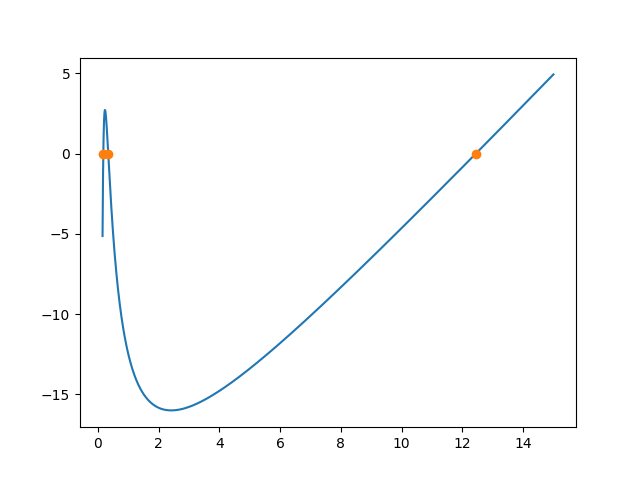
\includegraphics[scale=1]{Figures/01_1.png}
    \end{center}

    Note that the ideal gas law states that
    $V = \frac{nRT}{P} = \frac{0.08205 \times 313}{2} = 12.840825$ liters.
    This is very close to the first possible volume that satisfies the van der
    Waal equation, $12.442597$ liters.

  \item % #9 Done
    According to Archimedes' law, when a solid of density $\sigma$ is placed in a
    liquid of density $\rho$, it will sink to a depth $h$ that displaces an
    amount of liquid whose weight equals the weight of the solid.
    For a sphere of radius $r$, Archimedes law is
    \[
      \frac{1}{3} \pi \p{3rh^2 - h^3}\rho = \frac{4}{3}\pi r^3 \sigma
    \]
    Given $r = 5$, $\rho = 1$, and $\sigma = 0.6$, determine $h$.
    You may use any one of your methods (make clear in your writeup which one
    you are using, what initial guesses or intervals you are using, etc...).

    The following script uses the method in implemented in problem 7 to find the
    height of the sphere according to Archimedes' law.
    The script uses three different initial guesses and gives three different
    roots.
    The three initial guesses were -4, 13, and 5.67.
    \lstinputlisting[language=Python]{01_9.py}

    The output of this script is shown below.
    \begin{verbatim}
The possible depths of the sphere are 5.6706892285, -3.9760987462, and 13.3054095177
    \end{verbatim}
    \begin{center}
      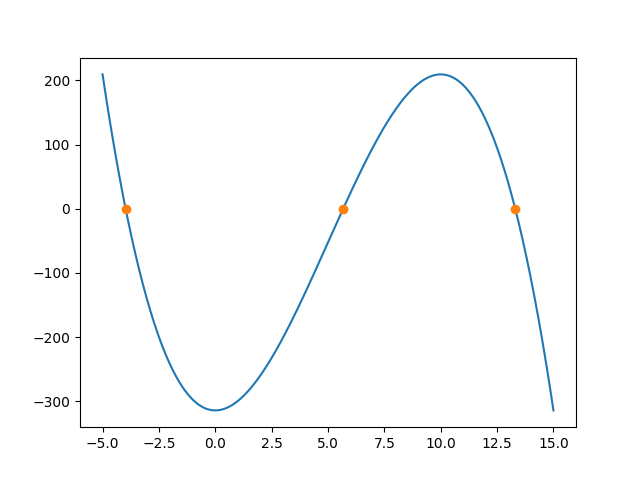
\includegraphics[scale=1]{Figures/01_2.png}
    \end{center}
\end{enumerate}
\end{document}
